\pdfminorversion=4
\documentclass[aspectratio=169]{beamer}
\usepackage{animate} % for animation
\usepackage{array,multirow,graphicx}
\usepackage{multicol}
\usepackage{etoolbox}
\graphicspath{{/home/fafaa/Documents/sinyal_dan_sistem/Slide/gambar}}
\setbeamertemplate{caption}[numbered]
\setbeamertemplate{section in toc}[sections numbered]

% Hide subsubsections from TOC, but keep PDF bookmarks with beamer
\hypersetup{bookmarksopen=true,bookmarksopenlevel=4}
\setcounter{tocdepth}{4}

\renewcommand{\figurename}{Gambar.}
\renewcommand{\tablename}{Tabel.}

\usetheme[pageofpages=of,	% String used between the current page and the
							% total page count.
			alternativetitlepage=true,% Use the fancy title page.
			titleline=true,
			titlepagelogo=OK-LOGO-ITK.jpg
%          	 titlepagelogo=fig/jaist_logo.png
			]{Torino}
			% change /beamerinnerthemefancy.sty to resize the logo
\usecolortheme{freewilly}

\makeatletter
\patchcmd{\beamer@sectionintoc}{\vskip1.5em}{\vskip0em}{}{}
\makeatother

\author{Mifta Nur Farid \\
	miftanurfarid@lecturer.itk.ac.id}
\title{TE201416: SINYAL DAN SISTEM}
\subtitle{SINYAL}
\institute{Teknik Elektro \\ Institut Teknologi Kalimantan \\ Balikpapan, Indonesia}
\date{\tiny Februari 26, 2020}

% The log drawn in the upper right corner.
\logo{
\includegraphics[height=0.13\paperheight]{OK-LOGO-ITK.jpg}}

\begin{document}

\begin{frame}[t,plain]
\titlepage
\end{frame}

\begin{frame}{Bahan Kajian}
%	\begin{multicols}{2} % Two columns for outline
    \tableofcontents[subsectionstyle=hide]
%	\end{multicols}
\end{frame}

\section{Sinyal sinusoidal}
\begin{frame}{Sinyal sinusoidal waktu kontinu}
	\begin{itemize}
		\item $ x(t) = A \cos(\omega_0 t + \phi) $
		\item $ A $ adalah amplitudo, $ \omega_0 $ adalah frekuensi dan $ \phi $ adalah fasa.
	\end{itemize}
	\begin{figure}
		\centering
		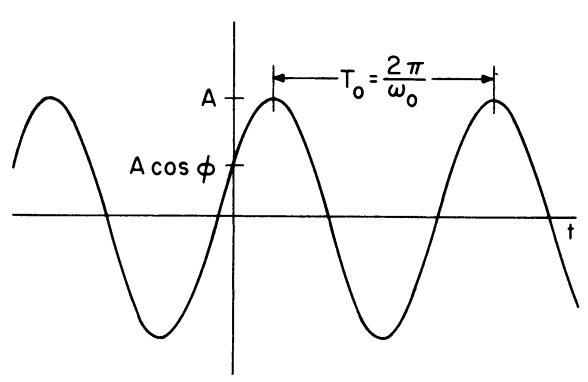
\includegraphics[height=0.6\textheight]{gambar/01.sinyal_sinusoidal_waktu_kontinu}
		\caption{grafik sinyal sinusoidal waktu kontinu} \label{sinusoidal}
	\end{figure}
\end{frame}

\begin{frame}{Periodik}
	\begin{itemize}
		\item Sinyal sinusoidal bersifat periodik
	\end{itemize}
	\begin{align*}
		x(t) &= x(t+T_0) \qquad \text{ periode } \triangleq \text{ nilai terkecil dari } T_0 \\
		A \cos[\omega_0 t + \phi] &= A \cos[\omega_0 t + \omega_0 T_0 + \phi] \\
		\\
		\text{syarat menghasilkan nilai yang sama} \rightarrow \omega_0 T_0 &= 2 \pi \text{; m} \text{m} \in \text{ bil. bulat}\\ 
		T_0 &= \frac{2 \pi \text{m}}{\omega_0} \implies \text{ periode } = \frac{2 \pi}{\omega_0} \\
	\end{align*}
	\begin{itemize}
		\item Jika kita perhatikan kembali gambar sebelumnya (Gambar \ref{sinusoidal}), maka pada periode $ \frac{2 \pi}{\omega_0} $ memiliki amplitudonya adalah sama
	\end{itemize}
\end{frame}

\begin{frame}{\textit{Time-shift}}
	\begin{itemize}
		\item \textit{Time-shift} dalam sinyal sinusoidal $ \iff $ perubahan fasa
	\end{itemize}

	\begin{align*}
		A \cos [\omega_0 (t + t_0) ] &= A \cos [\omega_0 t + \omega_0 t_0 ] \text{; } \omega_0 t_0 = \Delta \phi \\
		A \cos [\omega_0 (t + t_0) + \phi ] &= A \cos [\omega_0 t + \omega_0 t_0 + \phi]
	\end{align*}
\end{frame}

\begin{frame}{Genap (\textit{even})}
	\begin{itemize}
		\item Sinyal dikatakan bersifat genap (\textit{even}) jika dicerminkan pada titik nol memliki bentuk sinyal yang sama
		\item $ \phi = 0 \implies x(t) = A \cos(\omega_0 t) $	
	\end{itemize}
	\begin{figure}
		\centering
		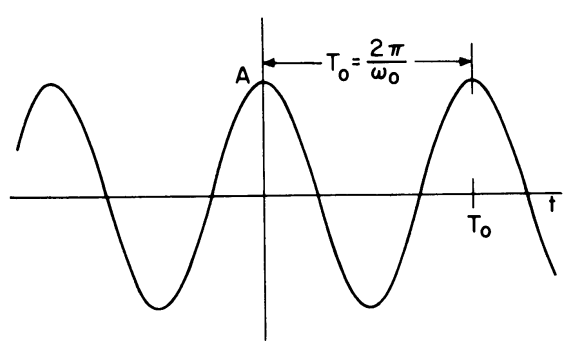
\includegraphics[height=0.35\textheight]{gambar/01.sinyal_genap}
		\caption{Sifat genap dari sinyal sinusoidal}
	\end{figure}
	\begin{itemize}
		\item Periodik : $ x(t) = x(t + T_0) $
		\item Genap : $ x(t) = x(-t) $
	\end{itemize}
\end{frame}

\begin{frame}{Ganjil (\textit{odd})}
	\begin{itemize}
		\item Sinyal dikatakan bersifat ganjil (\textit{odd}) jika dicerminkan pada titik nol memeliki bentuk sinyal yang berkebalikan terhadap sumbu-$ x $
		\item $ \phi = 0 \implies x(t) = A \cos(\omega_0 t) $	
	\end{itemize}
	\begin{figure}
		\centering
		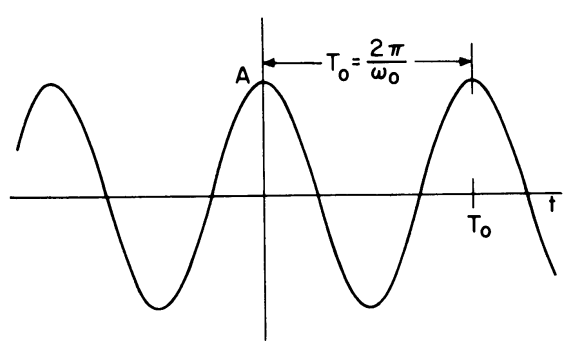
\includegraphics[height=0.35\textheight]{gambar/01.sinyal_genap}
		\caption{Sifat genap dari sinyal sinusoidal}
	\end{figure}
	\begin{itemize}
		\item Periodik : $ x(t) = x(t + T_0) $
		\item Genap : $ x(t) = x(-t) $
	\end{itemize}
\end{frame}

\end{document}

